      
               
                \begin{ledgroupsized}[r]{120mm}
                \footnotesize 
                \pstart                
                \noindent\textbf{\"{U}berlieferung:}   
                \pend
                \end{ledgroupsized}
            
              
                            \begin{ledgroupsized}[r]{114mm}
                            \footnotesize 
                            \pstart \parindent -6mm
                            \makebox[6mm][l]{\textit{L}}Notiz: LH XXXVIII Bl. 22. 1 Bl. 8\textsuperscript{o}. 3/4 S. Auf die obere H\"{a}lfte verteilt 7 Zeichnungen. Im oberen Viertel nicht von Leibniz' Hand folgende Notiz, die sich vorher auf dem Blatt befunden haben muss: 72 + 5 (100 + 77) ad rd ut 72 ad tang rad. Im unteren Drittel quergeschrieben \"{U}berlegungen zu mathematischen Reihen, die in Reihe VII ver\"{o}ffentlicht werden. R\"{u}ckseite leer.\\Cc 2, Nr. 1557 \pend
                            \end{ledgroupsized}
              
                            \begin{ledgroupsized}[r]{114mm}
                            \footnotesize 
                            \pstart \parindent -6mm
                            \makebox[6mm][l]{\textit{E}}\cite{00243}\textsc{Gerland} 1906, S.~208. \pend
                            \end{ledgroupsized}
                %\normalsize
                \vspace*{5mm}
                \begin{ledgroup}
                \footnotesize 
                \pstart
            \noindent\footnotesize{\textbf{Datierungsgr\"{u}nde}: F\"{u}r die Datierung sprechen inhaltliche Gr\"{u}nde, die sich aus der Methode ergeben, wie Seeleute die H\"{o}he von Himmelsk\"{o}rpern \"{u}ber dem Meer bestimmen. Davon ist insbesondere in der von Leibniz ausf\"{u}hrlich referierten Schrift Morins \textit{Scientia longitudinum} die Rede. Wie aus N. 10 hervorgeht, hat Leibniz den Titel im Sommer 1673 gelesen. Wir betrachten das vorliegende St\"{u}ck als eine Notiz zu dieser Lekt\"{u}re und orientieren uns f\"{u}r die Datierung an N. 10. Diese wird zudem durch \"{U}berlegungen zu mathematischen Reihen im unteren Teil des Blattes gest\"{u}tzt. \"{A}hnliche \"{U}berlegungen finden sich in \textit{LSB} VII, 4 N. 15 und 16, die ebenfalls zu dieser Zeit entstanden sind.}
                \pend
                \end{ledgroup}
            
                \vspace*{8mm}
                \pstart 
                \normalsize
            \begin{center}%\selectlanguage{french}
            [22 r\textsuperscript{o}] Comme les pilotes prennent les hauteurs sur mer.\end{center}\pend   \vspace{1.0ex}\pstart %\selectlanguage{latin}
              \begin{wrapfigure}{l}{0.58\textwidth}                    
              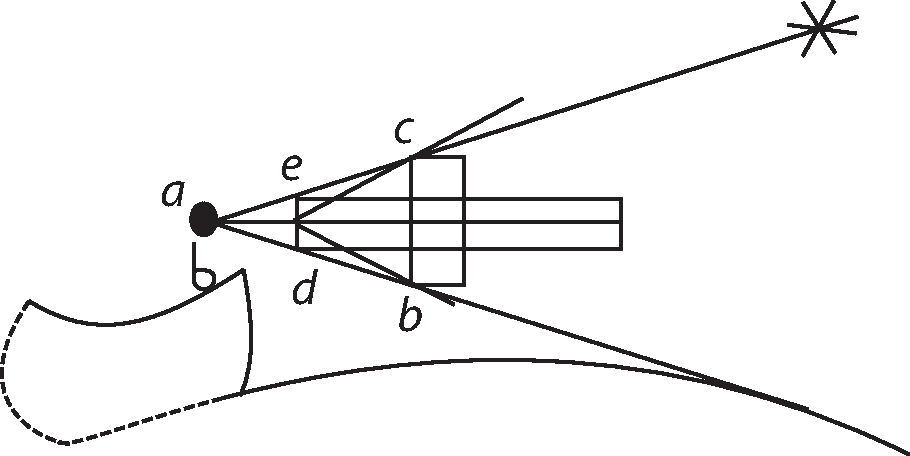
\includegraphics[width=0.58\textwidth]{images/38_22r3}
              \\\begin{center}\textit{[Fig. 1]}\end{center} 
              %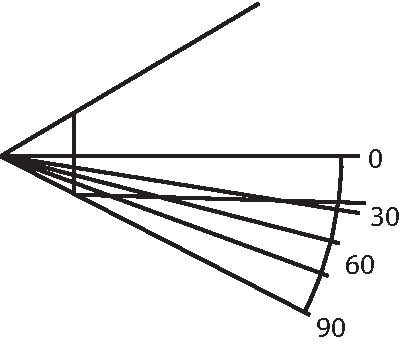
\includegraphics[width=0.5\textwidth]{images/38_22r2}
              %\caption{Bildbeschreibung}
              \end{wrapfigure}
            Primum male sumunt lineam horizontalem, aquam aspiciunt \`{a} fleur d'eau, sed ipsa primum altitudo  navis errorem facit. Deinde quod longe  importantius, usus instrumenti quod vocant l'arcbaleste\protect\index{Sachverzeichnis}{arcbaleste}, est corruptissimus.  Deberent inspicere ex centro \textit{a} cum per extremam spiciant  ut illi inspiciant \textit{db}, \textit{ec} separatim, at ipsi centrum ponunt in \edtext{media rectae} {\lemma{media}\Afootnote{ \textit{ (1) }\ arcus \textit{ (2) }\ rectae \textit{ L}}} \textit{ed}. \pend \pstart Methodum habeo perfecte observandi in navi, quantum ab homine possibile
              \begin{wrapfigure}{l}{0.3\textwidth} 
              \begin{center}                   
              
\includegraphics[width=0.2\textwidth]{images/38_22r1}
              \\\textit{[Fig. 2]}\\
              \vspace{0.5ex}                   
              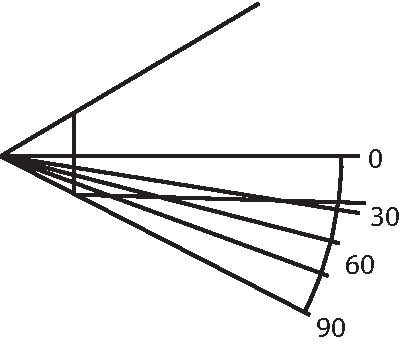
\includegraphics[width=0.3\textwidth]{images/38_22r2}
              \\\textit{[Fig. 3]}
              %\caption{Bildbeschreibung}
              \end{center}
              \end{wrapfigure}
            est. \newline Ope Instrumenti Thevenotiani \edtext{}{\lemma{Thevenotiani}\Bfootnote{\cite{00135}\textsc{M. Th\'{e}venot}, \cite{00135}\textit{Machine nouvelle}, \textit{JS}, 15. November 1666, S.~439\textendash 443.}} haberi potest linea horizontalis, inde forma quadam Camerae obscurae\protect\index{Sachverzeichnis}{camera obscura} portabilis adhibita, chartaque inolita eousque mutetur situs,  dum stella  quaesita in certo appareat puncto  chartae. Ubi ibi apparuit tacto  quodam Elaterio machinae partibus  stabilis quidam situs detur, quo facto habebitur angulus quaesitus. Hoc modo non opus est inspicere per dioptram\protect\index{Sachverzeichnis}{dioptra}, quo casu quaerere  difficile. At ipsam dioptram\protect\index{Sachverzeichnis}{dioptra} dirigere in stellam, non  inspiciendo per dioptram\protect\index{Sachverzeichnis}{dioptra} videtur adhuc difficilius sed  hoc invento emendatur.\pend \vspace{10mm}           
              \begin{center}
              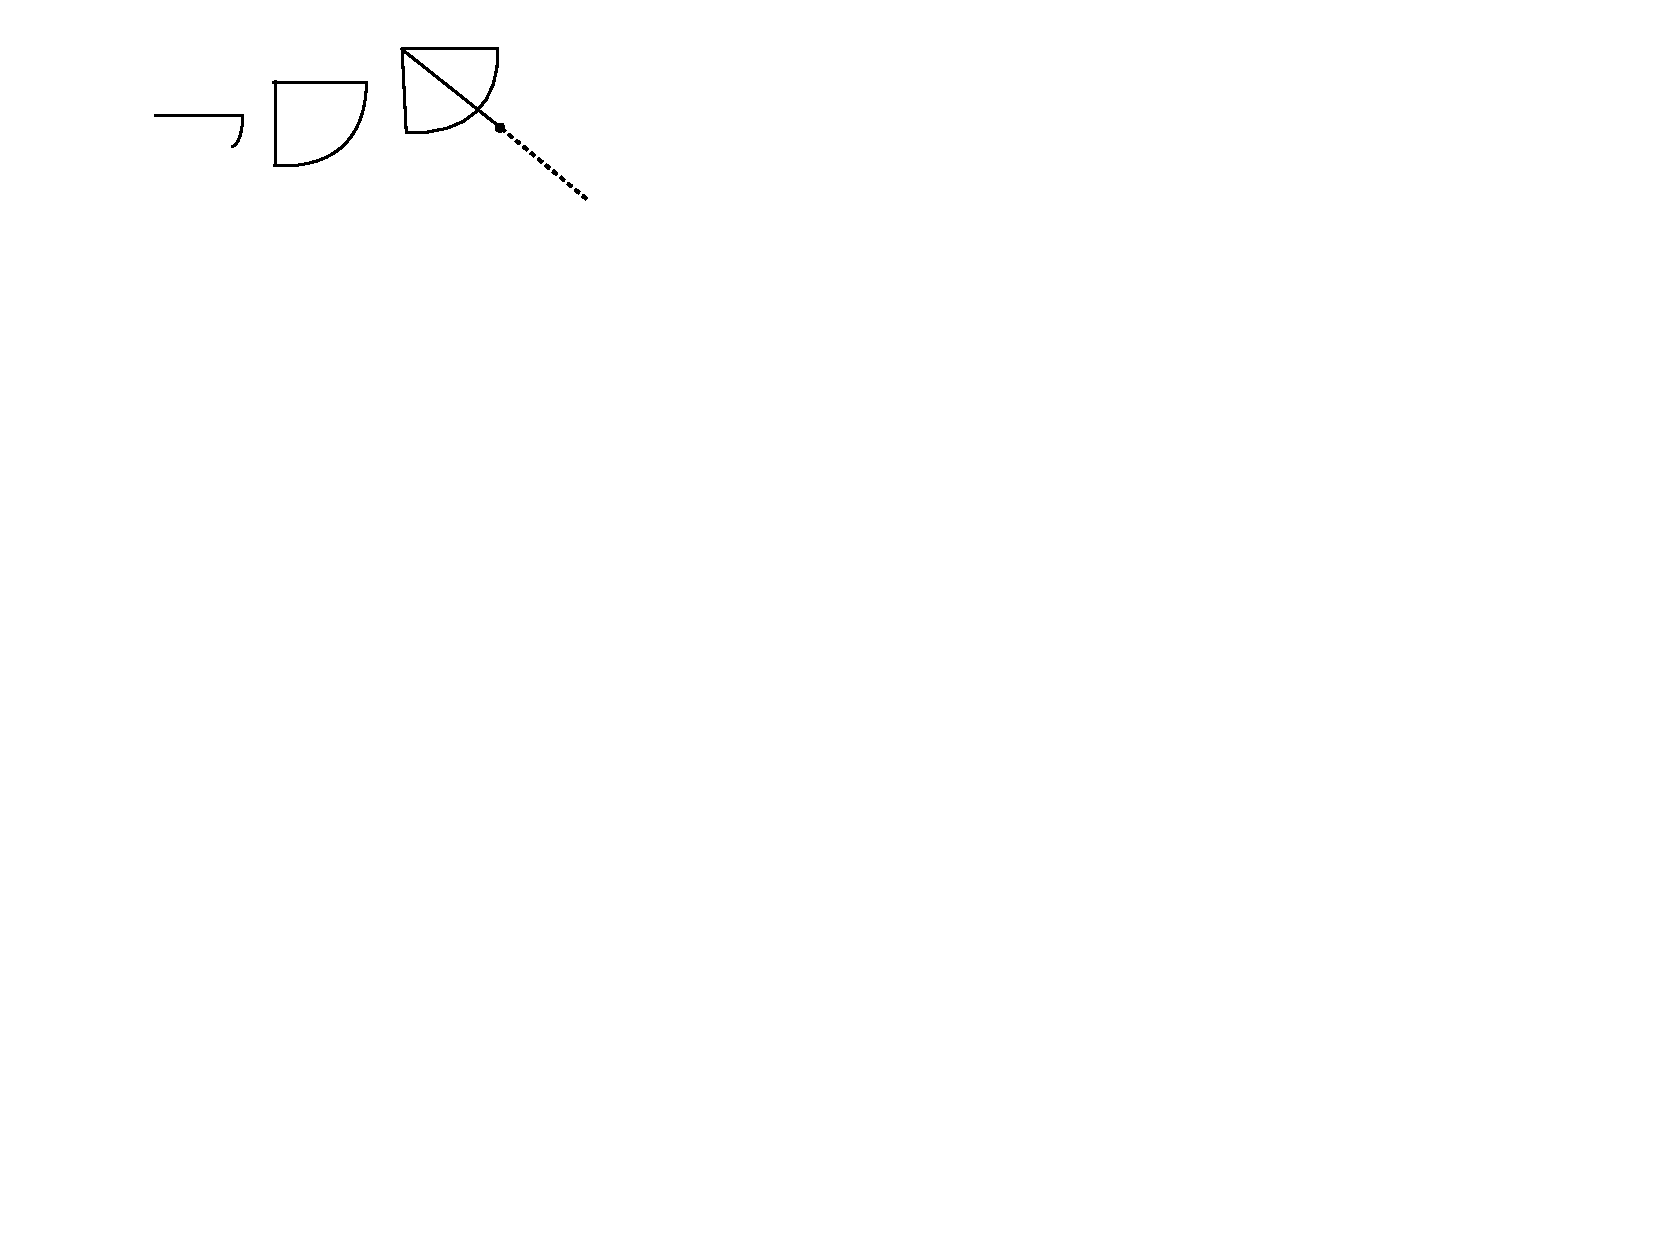
\includegraphics[width=0.5\textwidth]{images/38_22r456}
              \\  \textit{[Fig. 4]} \vspace{5mm}
              \\
              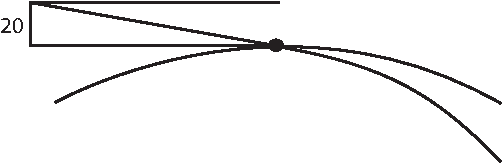
\includegraphics[width=0.5\textwidth]{images/38_22r7}
              \\ \textit{[Fig. 5]}
              \end{center}